\bf{Пример}

Пусть $N=4,$ $M=4,$ $U=[0,0,0,1],$ $V=[1,2,3,2],$ $A=1,$ $B=3,$ $S=1,$ и $T=3.$

Проверяющий модуль вызывает \t{find_pair(4, [0, 0, 0, 1], [1, 2, 3, 2], 1, 3).}

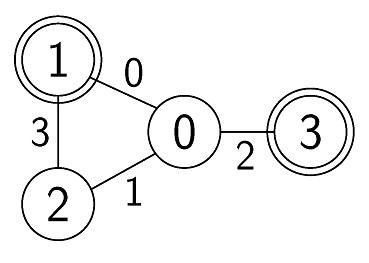
\includegraphics{image0.jpg}

На рисунке выше ребро с номером соответствует $i$ дороге $i.$ 
Некоторые возможные вызовы \t{ask} и соответствующие им возвращаемые значения показаны ниже:

\begin{tabular}{|c|c|}\hline
\bf{Вызов}&\bf{Возвращаемое значение} \\\hline
\t{ask([0, 0, 0, 0])}&$2$ \\\hline
\t{ask([0, 1, 1, 0])}&$4$ \\\hline
\t{ask([1, 0, 1, 0])}&$5$ \\\hline
\t{ask([1, 1, 1, 1])}&$6$ \\\hline
\end{tabular}

При вызове \t{ask([0, 0, 0, 0])} все дороги слабо загружены и пошлина для каждой из них равна $1.$ Самый дешевый путь из $S=1$ в $T=3$ --- это $1 \rightarrow 0 \rightarrow 3.$ Суммарная пошлина для пути равна $2.$ Таким образом, эта функция вернёт $2.$

Для правильного ответа процедура \t{find_pair} должна вызвать \t{answer(1, 3)} или \t{answer(3, 1)}.

Файл \t{sample-01-in.txt} в прилагаемом архиве соответствует этому примеру. В архиве есть и другие примеры входных данных.
